\documentclass{article}

%%%%%%%%%%%%%%%%%%%%%%%%%%%%%%%%%%%%%%%%%%%%%%%%%%%%%%%%%%%%%%%%%%%%
%%-----------------------PAGE SETTINGS----------------------------%%
%%%%%%%%%%%%%%%%%%%%%%%%%%%%%%%%%%%%%%%%%%%%%%%%%%%%%%%%%%%%%%%%%%%%
\usepackage[utf8]{inputenc}
\usepackage[margin=0.01cm]{geometry}

%%%%%%%%%%%%%%%%%%%%%%%%%%%%%%%%%%%%%%%%%%%%%%%%%%%%%%%%%%%%%%%%%%%%
%%--------------------------PREAMBLE------------------------------%%
%%%%%%%%%%%%%%%%%%%%%%%%%%%%%%%%%%%%%%%%%%%%%%%%%%%%%%%%%%%%%%%%%%%%
\usepackage{graphicx}
\usepackage{pdfpages}
\usepackage{anyfontsize}
\usepackage{setspace}
\usepackage{amsmath}
\usepackage{amsfonts}
\usepackage{amssymb}
\usepackage{natbib}
\usepackage{booktabs}
\usepackage{svg}
\usepackage{siunitx}

\definecolor{lightblue}{rgb}{0.23, 0.45, 0.57}
\usepackage[colorlinks=true,linkcolor=blue,allcolors=lightblue]{hyperref}
\usepackage[toc,page]{appendix}


%%%%%%%%%%%%%%%%%%%%%%%%%%%%%%%%%%%%%%%%%%%%%%%%%%%%%%%%%%%%%%%%%%%%
%%-----------------------CUSTOM COMMANDS--------------------------%%
%%%%%%%%%%%%%%%%%%%%%%%%%%%%%%%%%%%%%%%%%%%%%%%%%%%%%%%%%%%%%%%%%%%%
\newcommand{\textBF}[1]{%
    \pdfliteral direct {2 Tr 1 w} %the second factor is the boldness
     #1%
    \pdfliteral direct {0 Tr 0 w}%
}

\newcommand{\textDF}[1]{%
    \pdfliteral direct {2 Tr 0.2 w} %the second factor is the boldness
     #1%
    \pdfliteral direct {0 Tr 0 w}%
}


%%%%%%%%%%%%%%%%%%%%%%%%%%%%%%%%%%%%%%%%%%%%%%%%%%%%%%%%%%%%%%%%%%%%
%%-----------------------DOCUMENT BEGIN---------------------------%%
%%%%%%%%%%%%%%%%%%%%%%%%%%%%%%%%%%%%%%%%%%%%%%%%%%%%%%%%%%%%%%%%%%%%
\begin{document}

\begin{titlepage}
\thispagestyle{empty}
\title{

\includegraphics[width=19cm]{Extras/rug_fse_cs_logo.pdf} \\
\vspace{3cm}
\begingroup
\setstretch{4}\fontsize{38}{10}\selectfont\fontdimen2\font=0.8ex
\parbox{13.3cm}{\textBF{Feature selection \\performance assessment}} %%Title
\endgroup}
\date{July 2021}
\author{J.G.S. Overschie}
\maketitle
\vspace{-1.5cm}
\hspace{4cm}\parbox[b][15cm][b]{8cm}{\textDF{\large\setstretch{1.5}
MSc Thesis INMSTAG-08\\
% June 2020\\
Student: J.G.S. Overschie\\ %NAME
First supervisor: dr. G. Azzopardi\\
Second assessor: A.M.J.A. Alsahaf}}
\end{titlepage}
\newpage
\newgeometry{top=1in,bottom=1in,right=1.25in,left=1.25in} %Needed because margins were changed for titlepage

\hrule
\begin{abstract}
The evaluation of feature selection algorithms is a many-faceted problem, which has been conducted in different ways in the literature. With a unified theoretical framework lacking, authors resort to widely used methods of evaluation - which are not necessarily optimal. In this paper, all relevant aspects of the evaluation process are thoroughly analyzed, after which a set of sensible metrics is distilled. Using \textit{a priori} information about relevant features, promising metrics to measure feature subset quality include the ROC\-AUC- and mAP scores. Furthermore, measures of stability and statistical integrity testing are given. An implementation of the pipeline, fseval, is made publicly available. Finally, a quantitative experiment implements and discusses the newly proposed set of metrics, which shows the new metrics to be of value and able to foretell feature subset prediction performance.
\end{abstract}
\hrule
\begin{quote}
    
\end{quote}

\section{Introduction}
% Feature selection has had a role, but is becoming ever more important
Feature selection has since long played an important role in data mining and prediction tasks, where the removal of irrelevant or redundant features can decrease the required storage space of a dataset without decreasing prediction performance. Even, in some cases prediction performance can increase, due to less noise in the input signal. In the current age and time, however, feature selection is becoming ever more relevant - there now exist cases where it becomes unfeasible to store and process all features of a dataset in its entirety; even though computational power and storage space increase, the improvements in hardware performance are now outpaced by the ever-larger datasets available \citep{thomee2016yfcc100m}. Hence, there is a need for reducing dataset dimensions.

% Real life practical examples for large datasets
Datasets have grown in both dimensions and amount of samples over the last couple of decades (UCI repository growth \citep{alelyani2013feature}). Internet traffic increased, new and more accurate measuring devices came to market, and disk storage space became cheaper. Whilst in most areas both the amount of dimensions ($p$) and the amount of samples ($n$) increased, in some fields the amount of samples remains sparse relative to increasing dimensionality; bio-informatics, for example. Whilst the process of obtaining samples can still be intrusive, sensory devices got more accurate, causing more information to be available on a single sample. These datasets are of 'large $p$ - small $n$' shape ($p \gg n$), which are challenging to reduce dimensions for due to the small amounts of samples. These, and other dataset shapes can benefit from applying feature selection techniques. 

% Now, what the paper is about; feature selection **performance assessment**; what previous papers did
Existing literature on feature selection is extensive. Many methods exist, taking various approaches. What remains a common point of concern, however, is a consistent and reliable way to evaluate feature selection method performance. This need is expressed in several papers, e.g. 'a unifying theoretical framework is lacking' \citep{guyon2003introduction}. Most often, feature selection is applied to real-world datasets, after which the performance of a prediction task is assessed using labelled data. In this way, different feature selection methods would output different feature subsets which in turn would influence the validation predictor performance. The problem with this approach is that the evaluation becomes reliant on the choice of the validation predictor, as well as the fact that the 'correctness' of the chosen features is not taken into account. Commonly missing in papers is also an analysis on algorithm stability and a statistically sound argumentation for superiority. Therefore, a more controlled and more systematic way of arguing one method's performance over another is desired.

% This paper's goal
The goal of this paper is to provide an analysis on common ways of evaluating feature selection method performance, by discussing recent literature. With a better understanding of reasonable ways to argue for any given method, a distillation is then made to recommend a practical evaluation pipeline for feature selection methods.

% 2 ways. + scope
% TODO 3 contributions; theory, quantitative research, fseval. + scope
This research contributes in three ways. First, ways of effective feature selection performance assessment are explored, in which different ways of assessing performance in literature are compared and a reasoning is provided as to what metrics are sensible to use in various cases. Second, a quantitative research using the proposed set of metrics is performed, comparing various promising supervised feature selection methods for classification problems. In the empirical part of this research, \textbf{scope} was reduced to focusing on supervised feature selection for classification problems using datasets that exhibit 'conventional flat features' (terminology available in Chapter~\ref{sec:reducing-dimensions}). However, the proposed feature selection evaluation pipeline should also be applicable to evaluating unsupervised setups too. Last, the proposed pipeline was implemented in Python and published as a package on Github, allowing authors to easily implement the pipeline themselves.

% Table of contents
The paper is built up in several theoretical chapters, followed by quantitative analysis results, a discussion and a conclusion. Chapter~\ref{sec:reducing-dimensions} explains the basic feature selection process and lays out basic terminology. Chapter~\ref{sec:evaluation} discusses how to best evaluate feature selection performance, by first discussing the state of affairs and then proposing a new set of metrics to use in evaluation. Chapter~\ref{sec:experiment} walks through a quantitative experiment using the newly proposed set of metrics. Finally, Chapter~\ref{sec:conclusions-and-futurework} discusses directions for future work and concludes the research.

\section{Reducing dimensions}\label{sec:reducing-dimensions}
Among the subject of reducing dataset dimensions, there exist a common terminology that is used among the literature. Whilst some terminology is synonymous, other seemingly related terms mean different concepts entirely.

% Categories of dimensionality reduction / feature screening / etc.
\textbf{Feature selection} and \textbf{feature projection} are both terms relating to the concept of dimensionality reduction \citep{cunningham2007dimension}, however, there exists an important distinction between them. Whilst in the process of feature selection, relevant dimensions are sought and selected without altering their input values, in the process of feature projection (also called \textit{feature extraction}) data transformations are applied, mapping the original data onto a lower-dimensional space. Although the two the methods are different, the two aim to achieving the same goal, and are thus encountered in similar contexts. In this paper, the term \textit{feature selection} is used as a term to indicate the general process of obtaining a feature subset with reduced size without transforming the data - note that any feature selection method might transform the data in the algorithm however it likes internally - the stated terminology is only concerned with the eventual output of the feature selection algorithm.

Common methods of feature projection are \textit{Principle Component Analysis} (PCA) for the supervised case and \textit{Linear Discriminant Analysis} (LDA) for the unsupervised case. Both PCA and LDA take a statistical approach to detecting feature interactions, which not always results in an optimal feature set for prediction. Rather, machine learning techniques can be used to select a more optimal subset.

\subsection{Common approaches}
% Categories of FS; filter/wrapper/embedded/hybrid ; supervised/unsupervised ; classification/regression ; feature types
Methods can be roughly subdivided between filter-, wrapper- and embedded methods \citep{chandrashekar2014survey}, which lays out a common taxonomy within the field.

\textbf{Filter methods} use some scoring mechanism to compute 'usefulness' for each feature, without applying a learning algorithm. Having applied some ranking criterion, often a feature ranking is produced, after which some thresholding operation can be applied to select features. Although filter methods are often computationally light and do not overfit due to the absence of a learning algorithm, filter methods might miss out on more complex feature interactions, causing a non-optimal subset as a result. Also, choosing a suitable threshold to use can be difficult.

\textbf{Wrapper methods}, on the other hand, use some learning algorithm to determine a suitable subset of features. A search is conducted over the space of possible feature subsets, eventually selecting the subset that has the highest validation score in the test set using a chosen learner as a predictor. Characteristics that define wrapper methods lend themselves similar characteristics to traditional optimisation problems; although an exhaustive search might yield an optimal solution, such a solution might not always be feasible due to its great time complexity. For this reason, in some applications a liberal filter is applied first, before running a wrapper method.

\textbf{Embedded methods} seek to combine the training task and feature selection. Given some suitable learner, features are weighted during the training process, producing either a feature ranking or a feature subset afterwards. e.g. some learners compute feature importance scores as part of their training process, which can then be used in combination with some threshold to select relevant features. Having already trained the model, subsequent prediction tasks can benefit from increased prediction speed by using less data.

\textbf{Hybrid methods} is any method that is not classifiable by a single category, but rather lends from multiple categories. Hybrid methods can, for example, combine filter and wrapper methods \citep{hsu2011hybrid}, by first applying a computationally efficient filter and refining the result by using a wrapper method. Another paper \citep{das2001filters} describes its approach as hybrid due to both adding- and removing features in the feature selection process - exhibiting both forward- and backward selection at the same time. Lately research was also put into examining \textit{Ensemble} feature selection methods \citep{bolon2019ensembles}, which combines outputs of multiple selectors and decides useful features accordingly using some voting committee. Ensemble methods can be seen as hybrids or are seen as a category on its own.

\subsection{Types of features}
An important consideration in choosing a suitable feature selection for any task, is what structure the concerning data has, if any at all. Data might exhibit tree, graph, or grouped structures, which is essential information when detecting feature interactions and determining useful features. Support for structured data is relatively new in the field, and has not been an extensive point of concern for many feature selection algorithms in the past. Many traditional feature selection algorithms focused primarily '\textit{conventional flat}' features \citep{li2017feature}, in which the assumption is made that the data is independent and identically distributed (\textit{i.i.d.}). This assumption is widespread among many machine learning algorithms, though, since in many applications datasets are normalized to fit the i.i.d. condition before they are used.

Conventional data are opposed to more complex data structures, i.e. datasets with 'structured features', as coined by the proposed taxonomy from J. Li et al (2017) \cite{li2017feature}, but also to linked data and \textit{streaming data}. In streaming data, the quality of an initially selected feature subset can be improved as more data comes in, and a feature selection algorithm is able to benefit from a larger distribution of samples. Adapting existing feature selection algorithms to fit the demands of streaming data proved to be a non-trivial problem. Nowadays many companies and institutions have to deal with data volumes that easily exceed the boundaries of in-memory storage capacity - limiting the data scientist to train on only subsets of the entire datasets. Smart sampling is therefore needed to retain a representative sample distribution.

The scope of this research is limited to only the most common type of features, \textbf{conventional-, flat features} (\textit{i.i.d.}).

% \subsection{Useful features}
% what makes a feature useful?
% relevant, redundant, irrelevant

% \subsection{Learning supervision}
% supervised vs unsupervised FS

\section{Evaluating performance}\label{sec:evaluation}
% even though many papers use 'widely used' methods, they might be non-optimal
Evaluating the performance of feature selection algorithms is a non-trivial problem. Among a wide range of metrics, no consensus exists among researchers, leaving many papers to present outcomes in different ways \citep{guyon2003introduction}. Even though in absence of a single consistent evaluation pipeline across the field, many scholars adhere to methods that are 'widely used' \citep{solorio2020review} \citep{li2017feature}, there might be methods of evaluation that are more meaningful. % any widely adopted method can be sub-optimal.

\subsection{State of affairs}
Recommendations for metrics have been given in previous papers, most often when discussing future work. Arguments are made for relevant aspects to evaluate, such as in Chandrashekar (2013) \citep{chandrashekar2014survey}: \begin{quote}\textit{"a feature selection algorithm can be selected based on the following considerations: simplicity, stability, number of reduced features, classification accuracy, storage and computational requirements"}\end{quote}Of these aspects most proposals focus mainly on number of reduced features, classification accuracy and computational requirements. Let us explore what classifiers and corresponding metrics are used in papers across the field. Afterwards, evaluation aspects are covered that are not present in the aforementioned set.

\textbf{Supervised feature selection} is most commonly evaluated by running some predictor over the concerning dataset using the selected feature subset, obtaining the easily interpretable accuracy metric in the classification case. Predictors often used in the literature include k-NN \citep{al2020review} \citep{mafarja2020dragonfly}, SVM's \citep{chandrashekar2014survey}, Decision Trees \citep{li2017feature} and Naïve Bayes \citep{koller1996toward}. Metrics used are often classification accuracy or in some cases average error rate \citep{khurma2020evolopy}, validated using some $n$-fold cross validation, commonly 5- or 10-fold.

\textbf{Unsupervised feature selection} is often evaluated using a k-means predictor, as noted by Solorio-Fern$\acute{a}$ndez (2020) \citep{solorio2020review}, in which 68 papers were reviewed. Metrics include Clustering Accuracy (\textit{ACC}) and Normalized Mutual Information (\textit{NMI}). 

\textbf{Stability}, on the other hand, is not widely used in theoretical or quantitative argumentation. Even though stability was recommended as a relevant evaluation metric by Chandrashekar (2013), not many papers explicitly argue for the stability of their method; the metric is called an \textit{"overlooked problem"} in Chandrashekar (2013). In many papers this metric is still regarded as a future work for solidifying any experimental results - the development of algorithms that achieve both high classification accuracy and high stability is still seen as a 'challenging' problem by Tang et al (2015) \citep{tang2014feature}.

The trend seems to be turning though, with more authors becoming aware of the importance of stability. Our reliance on machine learning is ever-increasing, and so does the demand for interpretability and reliability of the algorithms. Take for example a bio-medical application, in which feature selection is used to select genes in a gene sequencing analysis. Any expert in this domain field will feel more confident if an algorithm produces stable results given a varying sample population. This is how we define stability: given small changes in the sample data, the output of a feature selection process ought to be stable, i.e. the sensitivity of the selector to data perturbations. This metric for measuring an ability to generalize to achieving consistency has been long taken into account into prediction tasks, but not in feature selection.

\textbf{Scalability} is another point of attention that only recently caught more attention. The extra demand of algorithms to allow for parallel execution has been imminent as data grew tremendously large. Even, multi-core processing can lack in terms of performance, hence introducing the need for algorithms that can run in distributed fashion. Distributing a dataset over multiple machines poses challenges to some existing methods, though. Some current methods require the 'full dimensionality' of the dataset to be available in-memory \citep{tang2014feature}. Yet, other methods require each sample to be visited multiple times, e.g. to apply a sample re-weighting strategy in order to converge. For these reasons, dividing any dataset workload onto multiple workers is a non-trivial problem; no generalized solution exists for cutting the dataset into chunks.

It is up to individual algorithms to find suitable ways of supporting parallel solutions and more importantly, support cases where data is too large to fit in-memory, i.e. apply distributed computing. Recent strategies overcome the issue of working with less samples by retaining only those samples that are most representative of the data - eliminating the need for working with a full sample population. Although few in numbers, there exist proposals for distributed dimensionality reduction methods \citep{JMLR:v21:19-537}, using 'divide-and-conquer' techniques. Aggregating disjoint results would make for a performance similar to that of a centralized solution.

\subsection{Meaningful evaluation}\label{sec:meaningful-evaluation}
Let us revisit and complement all previous theory, and extract a sensible evaluation pipeline to use. First, each evaluation aspect is treated separately, followed by a recommendation, then an overview is drawn of the entire proposed evaluation pipeline.

% review the paper that says "no single 'best' feature algorithm exists".

\subsubsection{Simulations}\label{sec:evaluation-simulations}
% we need a controlled environment
Many proposals test their validity on real datasets. Although testing on real datasets might feel more intuitive since it is also the eventual domain of application, they may not prove the best fit for feature selection method evaluation. With any dataset for which we cannot exactly control its properties, we are resorted to a smaller available set of validation measures, such as classification accuracy. However, introducing synthetically generated probe variables, or even generating all benchmark data synthetically can provide more reliable results in a controlled environment.

%... already pitched slightly by Guyon, e.g. "fake" variables.. + Solorio & Urbanowicz
\textbf{Partially synthetic} datasets are spoken of in literature since long, using datasets that are real but altered by injecting more data. In \citep{guyon2003introduction} the authors speak of 'probe variables', which are used to discard any variable that scores lower than any of the probes. If the probe variables are set to be random variables, a simple way is obtained to apply a threshold to cutting off features from the selected feature subset, i.e. by introducing known noise into the dataset we can construct more thoughtful cut-off thresholds.

\textbf{Completely synthetic} datasets, on the other hand, can allow for more sophisticated metrics to be used. Possibilities for new evaluation metrics are for example described in \citep{solorio2020review}: \textit{"Evaluation in terms of the redundancy of the selected features”} and \textit{“Evaluation in terms of the correctness of the selected features”}, the latter of which requires us to know what features are informative \textit{a priori} - which is accomplished with synthetic generation. Controlling all facets relevant to the quantitative analysis manually makes for a \textit{Simulation study}, which is argued for in \citep{urbanowicz2018benchmarking} as follows:

%... then move to Urbanowicz with examples from JMLR papers
\begin{quote}
    \textit{"Simulation studies such as these facilitate proper evaluation and comparison of methodologies because a simulation study can be designed by systematically varying key experimental conditions, and the ground truth of the dataset is known i.e. we know which features are relevant vs. irrelevant, we know the pattern of association between relevant features and endpoint, and we know how much signal is in the dataset."}
\end{quote}

Indeed there seems to be a trend toward using synthetically generated datasets. In a review paper \citep{bolon2013review} the authors argue that synthetically generated datasets can yield statistically sound results because of the fact no inherent noise or redundancy will obstruct the experiment process.

% explain what metrics we can now compute.
\textbf{A priori} knowledge of relevant features allows us to evaluate feature selection results in a more meaningful manner. Algorithm performance measurements can take advantage of using classification metrics familiar to many - see Section~\ref{sec:evaluation-statistical-tools} - which allows us to better understand any algorithm's selection process in comparison to doing unsupervised evaluation. Another benefit is gained by relying on a priori knowledge in the validation process, which is that the evaluation process is no longer dependent on the choice of the validation classifier. Removing the validation classifier from the evaluation process completely can make for a more universal way of evaluating feature selection methods: whilst previously reported feature selection method scorings were dependent on the validation classifier and would per definition not be comparable across papers, using a priori based metrics allows for better comparability across papers.

In other, more recent papers simulation studies are conducted as well \citep{JMLR:v21:18-567} \citep{JMLR:v21:19-071} \citep{JMLR:v21:19-537}, concluded by a small section depicting a 'real data analysis' to conclude the point. For these reasons, we recommend use of simulation studies to evaluate feature selection methods.

\subsubsection{Feature subset quality}\label{sec:evaluation-statistical-tools}
Based on the new assumption of knowing the groundtruth in the evaluation process, possibilities are opened for use of many common classification metrics to evaluate feature subset quality. One can now compute the ratio of 'amount of selected relevant features versus the total amount of relevant features present in the dataset' and the ratio of 'selected relevant features versus the total amount of selected features'; recall and precision respectively. The amount of 'true negatives' will be the amount of features that were not selected and are not informative - hence implicitly correctly identified as irrelevant. With recall and precision now available, also the f-scores can be computed, as well as the true-positive-rates, false-positive-rates and therefore the ROC curve and AUC-scores.

\textbf{Statistical metrics} used for machine learning evaluation can be formulated in such a way to be suitable in the context of a feature selection evaluation process. Given a feature subset computed by a feature selector, metrics can be defined as such:

\begin{table}[ht]
\begin{tabular}{llll}
 &  & \textit{Amount of} \\
True Positives & ($TP$): & selected 'informative', i.e. groundtruth features \\
False Positives & ($FP$): & selected 'uninformative', i.e. redundant/irrelevant features \\
True Negatives & ($TN$): & unselected uninformative features \\
False Negatives & ($FN$): & unselected informative features \\
\end{tabular}
\end{table}

Negatives are indicated as the remaining dataset features not in the feature subset, i.e. $Negatives = p - Positives$ where $p$ is amount of dataset features. Using the above definitions more sophisticated metrics can be defined:

\begin{table}[ht]
\begin{tabular}{llll}
$Recall$ & $= \frac{TP}{TP+FN}$ & or $True$ $Positive$ $Rate$&  \\
$Precision$ & $= \frac{TP}{TP+FP}$ &  &  \\
$False$ $Positive$ $Rate$ & $= \frac{FP}{FP+TN}$ &  & 
\end{tabular}
\end{table}

\textbf{ROC- and PR curves} can now be computed, using the above definitions. However, one must take into account the fact that any dataset is represented by multiple replicas - and insight on aggregated results are desirable. Therefore, a coherent way of computing the mean curve must be found. For the ROC curve, the process is straightforward - a mean curve can be computed by first interpolating each curve over a set of equally spaced false-positive-rate ($fpr$) interval steps, e.g. $\{fpr \mid fpr \in [0, 1]\}$ with 100 intervals, and then averaging the interpolated recall values. Given the aggregated ROC curve, the ROC-AUC metric can easily be computed. For the PR curves, however, the solution is less trivial - due to the non-monotonic nature of the curve 'wiggles' are commonplace. Applying linear interpolation is known to cause an overly-optimistic performance estimate \citep{davis2006relationship}. Therefore, a more sophisticated way of interpolation is required for PR curves.

\textbf{Interpolating a PR curve} was written about in \citep{10.5555/576628} and its proposed measure was described in \citep{everingham2010pascal}:

\begin{equation}
p_{\text{interp}}(r)=\max_{\tilde{r}: \tilde{r} \geq r} p(\tilde{r})
\end{equation}

The formula defines the interpolated precision, $p_{\text{interp}}(r)$, for any recall value as the maximum precision value of all observations at the first recall level to the right with non-null observations. Such 'non-null' precision observations are defined as $p(\tilde{r})$ with its recall level $\tilde{r}$. By means of this interpolation method, wiggles are overcome, yielding a more consistent curve.

\textbf{AUCPR}, or Area Under the Precision/Recall Curve is a useful metric to summarize PR curve performance. There exist multiple ways of quantifying the metric, however, as was shown in \citep{boyd2013area}, with methods yielding different levels of robustness in the estimation process. In the paper a range of methods are discussed, e.g. a Trapezoidal Estimator and Average Precision. The authors, Boyd et al, empirically validated method robustness and, among others, concluded \textit{Average Precision} ($AP$) to be effective. Since the metric is often used in literature and is robust, it is a sensible metric to express the AUCPR. It can be defined as \citep{zhu2004recall}:

\begin{equation}
\mathrm{AP} = \int_{0}^{1} p_{\text{interp}}(r) d r
\end{equation}

Which is an integral over the recall range of $[0, 1]$ to obtain the area under the precision-recall curve. A finite implementation is constructed by summing the areas under each separate precision plateau. The amount of plateaus is finite and are at the maximum the amount of possible recall values, which in turn are the amount of informative features. So, rather than having to approximate the area by computing areas at equally spaced intervals, in this fashion, we obtain an accurate estimate for the Average Precision. The finite average precision is defined as:

\begin{equation}
\mathrm{AP}=\sum_{k=1}^{n} P_{\text{interp}}(k) \Delta r(k)
\end{equation}

Where $n$ is the amount of precision plateaus and $k$ the current plateau, for which an interpolated precision is available as $P(k)$ and $\Delta r(k)$ the change in recall given the precision plateau.

\textbf{Aggregated PR curves} can now be obtained by computing the mean curve from all interpolated curves - similar to how the ROC curve was aggregated. Now, however, we do not require interpolation in the aggregation process since the PR curves were already interpolated at fixed recall points. To aggregate the $AP$ scores, one can take the mean of all replica $AP$ scores, more commonly referred to as the \textbf{$mAP$} score:

\begin{equation}
\mathrm{mAP}=\frac{1}{m} \sum_{i=1}^{m} \mathrm{AP}_{i}
\end{equation}

Here, $m$ denotes the amount of replicas ran for a specific dataset, with $AP_i$ be the average precision for the $i^{th}$ replica.

Using these metrics, a useful set of statistical tools are laid out for evaluating feature subset quality, and thereby also feature selection method performance. Rather than just using validation estimators to measure feature subset prediction power, by comparing against a groundtruth the feature selection method evaluation process itself became supervised - possibly providing the process with more meaningful feedback.

\subsubsection{Stability}\label{sec:evaluation-stability}
Stability is an integral metric of any algorithm, for in many applications, only robust algorithms can be systematically relied on. A measure for quantifying stability that comes easily to mind might be the Hamming distance between multiple pairs of algorithm runs, i.e. ran on the same dataset with varied sample populations. Indeed, in \citep{dunne2002solutions} a measure based on Hamming distance is proposed. Reports also exist on numerous other approaches, like an entropy based measure \citep{kvrivzek2007improving}, a measure based on the cardinality of intersection measure \citep{kuncheva2007stability} and a measure based on correlation coefficients \citep{kalousis2007stability}.

\textbf{Desired properties} of any measure are important to define in concrete manner. To compare the strength of any of these measures, the general objective for exactly what information we want to convey in a stability metric should be verbalized first. In \citep{mohana2016survey}, three desired stability metric properties are expressed: (1) \textit{Monotonicity}, (2) \textit{Limits} and (3) \textit{Correction for chance}. Given the proposed measures in the literature, only few measures satisfied all properties. In a more recent paper \citep{nogueira2017stability}, however, the authors extend the set of desired properties to include another two: (4) the stability estimator must be \textit{Fully defined} and (5) \textit{Maximum Stability $\leftrightarrow$ Deterministic Selection} - meaning that a maximum stability value should be achieved if-and-only-if all feature sets are exactly identical.

\textbf{A stability measure} was proposed in \citep{nogueira2017stability}, using the set of newly proposed desired properties. Having explored a statistically sound method to define a metric satisfying all five properties, the authors proposed a novel stability estimator:

% \citep{saeys2008towards}
% \citep{Khaire et al, 2019}

\begin{equation}\label{eq:stability-measure}
\hat{\Phi}(\mathcal{Z})=1-\frac{\frac{1}{d} \sum_{f=1}^{d} s_{f}^{2}}{\mathbb{E}\left[\frac{1}{d} \sum_{f=1}^{d} s_{f}^{2} | H_{0}\right]}=1-\frac{\frac{1}{d} \sum_{f=1}^{d} s_{f}^{2}}{\frac{k}{d}\left(1-\frac{\bar{k}}{d}\right)}
\end{equation}

Here, $\hat{\Phi}$ resembles the stability estimate. It takes as an input $\mathcal{Z}$, which resembles a collection of feature sets chosen by the designated feature selection algorithm. We define $\mathcal{Z}$ as $\mathcal{Z} = \{s_1,...,s_M\}$, where $s_i$ is one feature subset of size $d$ features, with $d$ the amount of dimensions of the dataset and $M$ the amount of bootstrap samples - i.e. the amount of replicate datasets with equal probability distribution and dataset properties used to validate stability. Furthermore, the authors define $s_{f}^{2}$ as the unbiased sample variance of the selection of the $f^{t h}$ feature and $\bar{k}$ as the average number of features selected over the M feature sets. Given this paper's goal, there is no necessity for going into further mathematical details - for this we refer to the paper itself.

What is important, is that this new measure satisfies all desirable properties for quantifying stability, as was proven in the paper. Accompanying the novel definition, are instructions for computing confidence intervals and for performing a hypothesis testing for comparing various method stabilities. Exploring feature selection stability values given a set of parameter choices not only allows for choosing better hyperparameters, but also allows for comparing stabilities over various feature selection methods. Therefore, we recommend use of the metric defined in (Eq~\ref{eq:stability-measure}) to quantify feature selection method stability.

\subsubsection{Algorithm complexity}
Another metric to be taken into account is algorithm complexity, which manifests itself in three interlinked aspects: time-, storage- and algorithm simplicity. Like the classical principle \textit{Occam's razor} implies - there at all times exist a preference for simpler models over more complex ones, especially in the case both accomplish the same feat. So, an understandable model is preferred that performs limited computational steps in order to restrain time- and storage complexity from rising too high.

Although measuring algorithm time- and storage requirements does provide some understanding, more insightful would be a theoretical description of the complexities in Big O notation. Theoretical complexities are harder to obtain though - leaving many authors to resort solely to measurements. Nonetheless, complexity analysis is recommended to be part of any feature selection method comparison, for it is a critical aspect to consider.

\subsubsection{Statistical integrity}\label{sec:evaluation-statistical-integrity}
Given the above discussed scalar metrics (mAP, ROC-AUC, Stability) for multiple feature selection methods computed for multiple datasets, a statistical test must be applied to provide convincing evidence for any algorithm's superiority. Like explained in \citep{demvsar2006statistical}, many papers make implicit hypotheses acclaiming improved performance over existing methods. Although chosen metrics might have been appropriate to statistically show performance gains as significant, results are less reliable when left unvalidated by a statistical test. Therefore, a statistical verification step is required in the feature selection evaluation process.

\textbf{Comparing multiple feature selectors} is a non-trivial problem, which can be seen as the problem of comparing multiple \textit{classifiers}. To compare multiple classifiers, \citep{demvsar2006statistical} recommends the Wilcoxon signed ranks test for comparison of two classifiers and the Friedman test for comparison of more classifiers given multiple datasets. Accompanying the Friedman test, it is recommended to perform corresponding post-hoc tests, such as the Nemenyi test \citep{nemenyi1963distribution}. The usually popular ANOVA test was advised against because, given the context of machine learning, ANOVA assumptions are violated, e.g. ANOVA assumes samples are drawn from normal distributions and the requirement of random variables having equal variance.

A \textbf{Wilcoxon signed ranks test} and the \textbf{Friedman test}, are for these reasons recommended, for two- or more methods respectively, to statistically verify significant differences in performance of feature selection algorithms over the other using some summarizing scalar per feature selection method per dataset. The Friedman test is recommended to be accompanied with a post-hoc test, like Nemeyi's post-hoc test.

\subsubsection{Pipeline}
All facets of meaningful evaluation were discussed and several recommendations were made. Wrapping up, a recommendation for an entire evaluation pipeline is given.

\textbf{Recommendations} for meaningful feature selection evaluation are as follows. (1) First of all, it is recommended to use synthetic datasets, such that informative features are known \textit{a priori} and datasets can be carefully designed to answer specific research questions, such as algorithm scalability or their ability to detect complex feature interactions. (2) Secondly, using now available groundtruth information, evaluation is recommended to benefit from analyzing common machine learning metrics, like the ROC- and PR curve, as well as summarizing metrics like the AUC- and mAP scores. (3) Third, stability should be measured using the tailor-made proposed measure from \citep{nogueira2017stability}. Note that computing algorithm stability does not require the groundtruth. (4) Fourth, algorithm complexity should be assessed in three different perspectives: simplicity, time complexity, storage requirements. A theoretical analysis is preferred. (5) Last, conclusions can be drawn by summarizing all computed metrics in a statistical verification test, using either the Wilcoxon signed ranks test or the Friedman test accompanied with the Nemenyi post-hoc test. Having statistically verified the results, a more scientifically reliable conclusion can be drawn.

\textbf{An implementation} of the proposed evaluation pipeline was built as part of the research. The framework implements many of the steps required in perform meaningful evaluation and is publicly available on Github \footnote{\url{https://github.com/dunnkers/fseval}}.

% \section{Method}
\section{Experiment results and discussion}\label{sec:experiment}
Using the newly defined set of metrics for evaluating feature selection methods, an quantitative study was conducted. In compliance with the idea of doing a simulation study, synthetic datasets were used. In this study, 76 synthetically generated datasets from \citep{urbanowicz2018benchmarking} are used, for which each 24 \textit{replicas} are considered - duplicate datasets but with different sample populations. The synthetic datasets cover various factors of influence to the feature selection task, like missing data, noise levels, sample sizes, dataset dimensionality and the types of feature interactions. All datasets possess a ground truth accordingly, which is resembled by the informative features an algorithm should select.

Testing was conducted on a selection of 4 supervised feature selection methods, using a mixed bag of methods that produce either a \textit{feature ranking} or a \textit{feature subset}. Other notable differences methods that exhibit \textit{stopping criteria} versus ones that do not, as well as forward- versus backward selection. The lineup is described as follows:

\begin{itemize}
    \item \textbf{ExtraTrees} \citep{geurts2006extremely}: ExtraTrees is a generic classifier used in a wide spectrum of applications, which works by creating an ensemble of (extremely) randomized trees. To use ExtraTrees as a feature selector, the feature importance scores are used to generate a ranking. This ranking is then reduced to a feature subset by cutting off features below the mean feature importance score, i.e. a threshold value defined as $\alpha = \frac{1}{p}\sum^{p}_{f=1}w_f$ and its feature subset as $\{f  \mid  w_f \geq \alpha\}$, where $p$ is the amount of features, $w_f$ is the $f^{th}$ feature importance score. 
    
    Configuration for ExtraTrees was set to use 50 estimators, all other settings were otherwise set at the scikit-learn \citep{pedregosa2011scikit} default. Since the feature importance scores are thresholded at the mean, the method produces not a ranking, but a \textbf{feature subset}.
    
    \item \textbf{FeatBoost} [undisclosed]: FeatBoost is a greedy forward feature selection algorithm proposed by Alsahaf et al in 2020, based on a sample re-weighting strategy. FeatBoost requires one to choose two estimators as hyperparameters: one estimator is used for the internal boosting process, and should expose feature importance scores, whilst another is used to validate some selected feature subset.
    
    Configuration was set such to explore 3 different hyperparameter settings: (1) First, a baseline configuration, referred to as simply '\textit{FeatBoost}'. FeatBoost using 'max features' set to 20 and the 'siso ranking size' set to 5 if amount of features $p \leq 100$ or set to 10 if amount of features $p > 100$. Furthermore, two XGBoost classifiers are used with 200 estimators and a max depth of 3. (2) Second, '\textit{FeatBoost w/1-NN}'. Same as the former, but with k-NN ($k = 1$) as a validation classifier. (3) Third, '\textit{FeatBoost Deep}'. Same as first, but both XGBoost classifiers having an increased maximum depth of 6. FeatBoost produces a \textbf{feature subset}.
    
    \item \textbf{MultiSURF} \citep{urbanowicz2018benchmarking} \citep{urbanowicz2018relief}: MultiSURF is related to the original Relief algorithm \citep{kira1992feature} and was first proposed in a benchmark paper for Relief-Based algorithms by Urbanowicz et al, in 2018. In the benchmark paper, amongst a selection of Relief-Based algorithms in a comprehensive, MultiSURF was recommended as an overall good performer.
    
    Configuration for MultiSURF was set such to rank the entire set of features, otherwise all other settings lay at default. Subsequently, the MultiSURF 'top features' attribute was used to produce a \textbf{feature ranking}.
    
    \item \textbf{Recursive Feature Elimination (RFE)} \citep{guyon2002gene}: In RFE, features with low feature importance scores are pruned away in step-wise manner, starting with the set of all features, i.e. using backward selection. The algorithm must be configured using an estimator exposing its feature importance scores, requesting new importance scores every step, iterating until a desired amount of features is selected.
    
    Configuration: RFE was configured using a XGBoost classifier configured exactly like in FeatBoost's configuration (1) and was set to eliminate features until the subset size is of length 1. Also, RFE was configured such, that in each 'elimination' round, 2 features are eliminated. Then, RFE's exposed ranking attribute is used to produce a \textbf{feature ranking}.
\end{itemize}

Analysis is split up in various sections. First, an empirical perspective will provide insights on feature selection method performance on various dataset themes, given the previously discussed metrics. Finally, after all dataset themes have been discussed, statistical hypothesis testing will be applied.

\subsection{Empirical observations}
Although testing was conducted on many datasets, it is sensible to first explore effectiveness of various metrics given a tangible example. The '\textit{3-way Pure Epistasis}' dataset was benchmarked at only 1 configuration, and hence lends itself well to a more thorough analysis. This first analysis is walked through in detail - once we established more trust in the chosen metrics, other datasets with more configurations can be analyzed en masse.

\subsubsection{3-way Pure Epistasis}
The 3-way Epistasis dataset records genetic information regarding Epistasis, which is a phenomenon in evolutionary biology describing how the mutations of one gene are dependent on other genes being mutated or not. In this case, 3-way interactions are considered - which also means that there exist 3 predictive features in the dataset. Another dataset property is 'heritability', which is a genetics term that in this context can be seen as the 'signal magnitude' \citep{urbanowicz2018benchmarking}. Heritability $h = 0$ resembles complete noise whilst a clean dataset is defined with $h = 1$, which in case the dataset is completely clean could theoretically lead to flawless predictions. For '\textit{3-way Pure Epistasis}' the heritability value is $h = 0.4$. Furthermore, the dataset is of dimensionality $p = 20$ and $n = 1600$. Like all other datasets, the dataset contains 24 replicas all generated using the same properties but exhibiting a different sample population.

\begin{table}[ht]
\centering
\begin{tabular}{@{}lllllllllllllll@{}}
\toprule
Feature Rank  & 1  & 2  & 3  & 4 & 5  & 6  & 7 & 8 & 9  & 10 & 11 & 12 & 13 & 14 \\ \midrule
Feature Index & \textbf{19} & 16 & 15 & 2 & \textbf{17} & 14 & 6 & 8 & 12 & \textbf{18} & 7  & 10 & 11 & 3  \\
Informative?    & \textbf{Y}  & N  & N  & N & \textbf{Y}  & N  & N & N &  N & \textbf{Y}  & N & N & N  & N   \\ \bottomrule
\end{tabular}
\caption{Output for the ExtraTrees feature selector using a mean-importance score threshold, ran on the '3-way Pure Epistasis' dataset, replica 1. }
\label{tab:3way-replica1}
\end{table}

\autoref{tab:3way-replica1} presents the \textbf{raw output} of 1 feature selection algorithm, ExtraTrees, given 1 replica. The algorithm constructed a subset with 14 features and managed to select all informative features, however, uninformative features were selected, too. Like argued in Section~\ref{sec:evaluation-statistical-tools}, there exist various ways to quantify performance. Let us explore several.
%ways to quantify performance are to reward selecting useful features and penalise selecting useless ones. To express these measures, Recall and Precision curves can be useful.

\begin{figure}[ht]
\centering
\includesvg[width=0.49\textwidth]{img/3way_repl1pr.svg}
\includesvg[width=0.49\textwidth]{img/3way_etpr.svg}
\caption{\textbf{Left}: Both precision and recall plotted against feature ranking. Metrics are raw unterinpolated data, for ExtraTrees, replica 1. \textbf{Right}: Interpolated Precision/Recall curve for ExtraTrees, all replicas. \textbf{Both} display the '3-way Pure Epistasis' dataset, for the ExtraTrees feature selector. }
\label{fig:3way_repl1pr_etpr}
\end{figure}

\autoref{fig:3way_repl1pr_etpr} depicts \textbf{Precision and Recall} metrics, for ExtraTrees. The left-hand plot depicts 1 replica and uses the data in \autoref{tab:3way-replica1} and the right-hand plot depicts all replicas. Whilst recall rewards an algorithm for selecting informative features in monotonically increasing fashion, precision both rewards and penalises. Whenever after a series of unsuccessful iterations, a useful feature was selected, precision jumps up - causing a 'wiggle' in the chart as theoretically explained in Section~\ref{sec:evaluation-statistical-tools}. For this reason interpolation was applied as according to the proposed evaluation pipeline, as seen on the right plot. Also on the right plot are text annotations, indicating how many replicas support the mean-PR curve at various points, i.e. not all replicas manage to select all informative features. In scenarios as such, where only several of the replicas manage to select all informative features, the mAP scores is still a representative summary of all replicas: the mAP score is computed as the mean of all \textit{Average Precision} scores, not the Area Under the Curve - one way to think of it in this case is as a weighted AUC score.

\begin{figure}[ht]
\centering
\includesvg[width=0.49\textwidth]{img/3way_roc.svg}
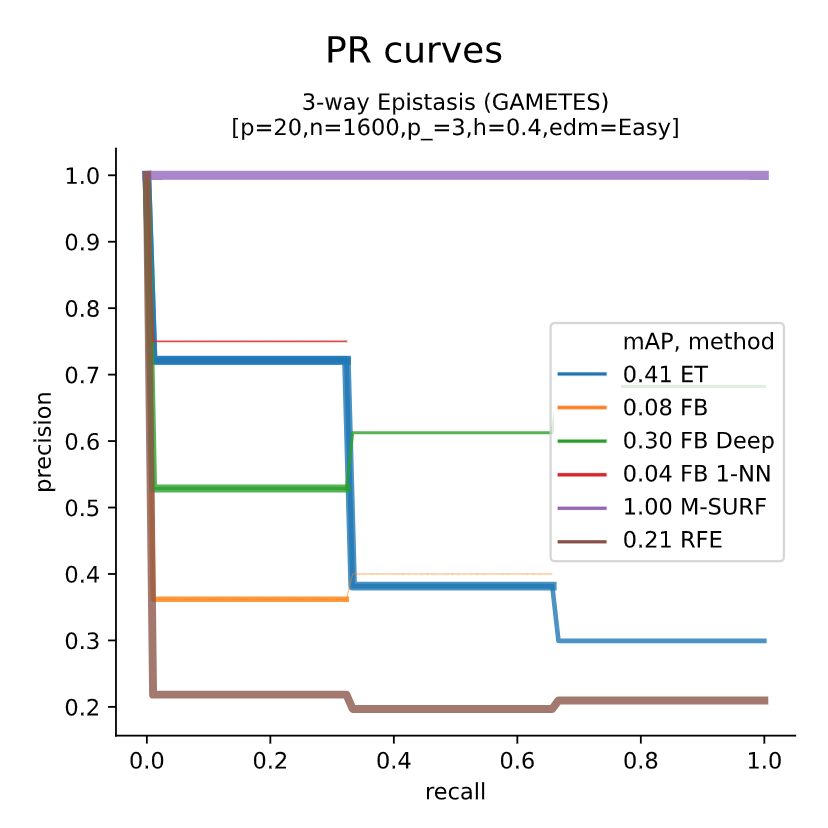
\includegraphics[width=0.49\textwidth]{img/3way_pr.png}
\caption{All ranking methods depicted in both the ROC- and (interpolated) PR space, for the '3-way  Pure  Epistasis' dataset. Accordingly to the ROC- and PR curves, respectively the ROC-AUC and mAP scores are attached.}
\label{fig:3way_rocpr}
\end{figure}

\autoref{fig:3way_rocpr} depicts \textbf{ROC- and PR curves} for all ranking methods. Whilst in the PR space algorithms are penalised for selecting useless features, in the ROC space algorithms are only rewarded (monotonically increasing) for selecting the right features, as fast as possible: the false-positive-rate will increase when selecting uninformative features, with the true-positive-rate only increasing when selecting informative features. It can be observed that in this behavior, stopping criteria are not taken into account - which the PR curve does manage to do: whilst in the ROC space RFE is only moderately penalised for selecting many false positives before selecting true positives, RFE relatively scores considerably worse in the PR space. It should be noted, though, that the PR curves might be overly optimistic due to the interpolation applied: all curves start by default at the (0 recall, 1 precision) point. This can clarify the perfect scoring for MultiSURF in the mAP score but not the ROC-AUC score. In the PR plot, lines of varied thickness are shown. Like explained in \autoref{fig:3way_repl1pr_etpr}, different PR 'plateaus' have different levels of replica support for their lines. The thicker the lines is, the more replicas support the line. This can help interpret, for example, the result of \textit{FeatBoost 1-NN}, where very few replicas managed to get a reasonable score, resulting in a thin line, accompanied by a low mAP score.

\begin{figure}[ht]
\centering
\includesvg[width=0.6\textwidth]{img/3way_stab.svg}
\caption{Stability versus Maximum feature subset size, depicted for all ranking methods for the '3-way  Pure  Epistasis' dataset.}
\label{fig:3way_stab}
\end{figure}

\autoref{fig:3way_stab} depicts the \textbf{Stability} metric, using the measure as explained in Section~\ref{sec:evaluation-stability}. Since the metric requires feature subsets rather than feature rankings, feature rankings are cut off at various points of maximum subset sizes, $k$. In the figure, stabilities have been computed for cut off points $k \in [1, 10]$. It can be observed that only MultiSURF produced a reasonably stable subset, peaking out at 3 features - which is consistent with the amount of predictive features of 3. Raw data shows us that indeed MultiSURF produced a completely stable subset at a subset size of 3 - selecting all informative features in all replicas. Lower stability in smaller subset sizes are due to the algorithm selecting informative features in different \textit{order}, i.e. there exist no ranking preference amongst the informative features themselves.

\begin{figure}[ht]
\centering
\includesvg[width=\textwidth]{img/3way_val_knnxgb.svg}
\caption{Classification Accuracy versus Feature Subset size, for the '3-way  Pure  Epistasis' dataset. Each replica produced 5 measurements with 5-fold CV. Results were averaged over 24 replicas, with the replicas partaking in the averaging process indicated by line width. Subsets were constructed by iteratively adding features of lower ranking scores for feature rankings, and similarly by adding features to a feature subset until its full size is reached.}
\label{fig:3way_val_knnxgb}
\end{figure}

\autoref{fig:3way_val_knnxgb} depicts \textbf{Classification Accuracy} scores for all ranking methods. The charts should not function as a general performance measure, like argued in Section~\ref{sec:meaningful-evaluation}, the charts are included, however, to convince the reader of the evaluation correctness of the previous steps: the previously shown metrics should be able to show what feature selection methods constructed powerful feature subsets and should hence perform well in any subsequent prediction task. Two predictors are considered: \textit{k-NN} ($k = 1$) and \textit{XGBoost}. For results of \textit{Gaussian Naïve Bayes} and  a (linear) \textit{Support Vector Machine}, see Appendix~\ref{sec:appendix-a}, \autoref{fig:3way_val_svmgnb}. All ran at default hyperparameter values.

Careful interpretation of the plot (\autoref{fig:3way_val_knnxgb}) is required: the process of aggregating the classification accuracy curve over various runs is open to graphical deceptions similar to what is seen in the Precision/Recall curves. Possible distortions are rooted in various algorithm runs stopping at different subset sizes due to stopping criteria, giving outliers possibility to distort the mean classification accuracy value. Whilst for the P/R curves it is possible to resort to the mAP metric, in a classification accuracy lineplot the supporting 'weight' of the mean curve is not directly visible. Therefore, in \autoref{fig:3way_val_knnxgb}, a 'line width' dimension was added, resembling the replica \textit{support} the mean curve has. A thicker curve means more replicas supporting the curve. It can be observed that MultiSURF performs well across all replicas - all replicas were instructed to rank all the features. For FeatBoost Deep, however, there exist outlier results with very little support - which is where, if simply the mean were taken, the mean curve would have been distorted. Curve support is weighted heavily, though, since according to the mAP and ROC-AUC scores, ExtraTrees evaluates higher, although in this validation stage it becomes clear that ExtraTrees does not perform so well - but it does so more consistently, i.e. with more curve support. According to what the earlier evaluation metrics were able to tell- the mAP and ROC-AUC scores represent feature selection method performance reasonably well.

\textbf{To summarize} all observations, mAP and ROC-AUC scores are able to foretell feature subset performance in a classification scenario. Much weight is put to the amount of replicas reaching their respective recall, precision or classification accuracy scores - which is in fact, sensible: an algorithm to perform well, but inconsistently, would have insufficient stability to be reliable and should thus score lower on feature selection evaluation metrics. In order to analyze other dataset themes \textit{en masse}, a representative choice has to be made between the various metrics, initiating the need to answer an important question: which plot best resembles feature selection algorithm performance?

Because of the ambiguity of the replica curve support that exists in the PR curves, in the further evaluations of other datasets solely ROC curves will be used. Even though this ambiguity has been tried to made visible, for example by means of text labels in \autoref{fig:3way_repl1pr_etpr} or by means of curve thickness in \autoref{fig:3way_rocpr}, still the lines do not faithfully represent the actual (consistent) performance and might therefore be misleading. It must be noted that the ROC curve might be overly-optimistic w.r.t. algorithms that have no stopping criteria - this can, however, be compensated by including the $mAP$ metric in a later analysis stage. The $mAP$ scores do faithfully represent performance over all replicas and will later be used in the statistical integrity testing section. Note that another solution would be to normalize replica subset sizes to be of equal length, e.g. by cutting off at a certain threshold or fixed length, or, to instruct feature selection algorithms to select a specific number of features - see Future work, Section~\ref{sec:future-work}. That said, due to the reasons above, in the remainder of analysis ROC curves will be used.

\subsubsection{Main Effects}
In the '\textit{1 Main Effect}' dataset theme there exist a single informative feature, that should be relatively easy to detect in comparison to feature interactions.

\autoref{fig:1_main_effect} depicts ROC curves for the given dataset theme. It can be observed that all algorithms perform decently well, except for \textit{FeatBoost 1-NN}, which seems to miss the informative feature in some cases.

\begin{figure}[ht]
\centering
\includesvg[width=\textwidth]{img/1_main_effect.svg}
\caption{ROC curves for '\textit{1 Main Effect}' dataset theme. 8 configurations were tested, with varying heritability and model difficulty levels (\textit{edm} in plot).}
\label{fig:1_main_effect}
\end{figure}

\subsubsection{2-way Epistasis}
The '\textit{2-way Epistasis}' dataset represent 2-way feature interactions and are hence more difficult than the a 1 main effect.

\autoref{fig:2way_epi} depicts ROC curves for 2-way epistasis. Immediately visible is the worsened performance in the 2-way interactions in comparison to 1 main effect. All algorithms seem to have difficulties with the hard models, although the FeatBoost algorithm configurations have most difficulty with high-noise (low heritability), hard models.

\begin{figure}[ht]
\centering
\includesvg[width=\textwidth]{img/2way_n=200.svg}
\caption{ROC curves for '\textit{2-way Epistasis}' dataset theme. 8 configurations of varying heritability and model difficulty levels were tested, with 4 different configurations of amount of samples. $n=200$, $n=400$, $n=800$, $n=1600$. See Appendix~\ref{sec:appendix-a}, \autoref{fig:2way_epi_large_samplesizes} for plots with $n=400$ and $n=1600$.}
\label{fig:2way_epi}
\end{figure}


\subsubsection{XOR benchmarks}
The XOR models are 'clean' datasets, which means the datasets are generated without any noise using a heritability parameter of ($h = 1.0$). The models include from 2 up to 5 informative features, influencing the difficulty of detecting the interactions.

\autoref{fig:xor_benchmarks} depicts ROC curves for XOR benchmark models. An interesting observation is that MultiSURF performance, which has previously been very steady, plummets quickly when the amount of feature interactions is increased. Although its AUC is still higher than the FeatBoost methods, it comes at a large false-positive-rate. ExtraTrees performance ranks highest for the high amount of feature interactions ($p_ = 5$), which might imply that ExtraTrees is better able to detect more complicated feature interactions. 

\begin{figure}[ht]
\centering
\includesvg[width=\textwidth]{img/xor_benchmarks.svg}
\caption{ROC curves for '\textit{XOR Benchmarks}'. For the theme there exist 4 different models, with 4 different amount of informative features ranging from $p\_= 2$ to $p\_ = 5$, exploring algorithm performance under higher-order interactions.}
\label{fig:xor_benchmarks}
\end{figure}

\subsubsection{Total number of Features}
Lastly, a dataset theme varying the total amount of dataset features whilst keeping other variables constant. Up until now all other datasets had a relatively small amount of features, which allowed us to answer questions about the types of complexity different feature selection algorithms can handle, but not exactly about \textit{scalability}.

\autoref{fig:total_features} depicts ROC curves for Total Number of Features datasets. For most feature selectors, an increased number of features has a tremendous impact on the quality of the chosen subsets. Raw data reveals that given the high feature dataset ($p = 10000$), all FeatBoost variants have their performance significantly impacted by both stopping early (subset sizes range from about 1 to 7) without having selected any correct features.

\begin{figure}[ht]
\centering
\includesvg[width=\textwidth]{img/total_features.svg}
\caption{ROC curves for the '\textit{Total Features}' dataset theme. Other dataset parameters (\textit{Easy} model difficulty, $h = 0.4$) were kept constant, whilst varying the amount of dimensions.}
\label{fig:total_features}
\end{figure}

\subsubsection{CPU timings}
\autoref{fig:cputime} depicts CPU timings for the Total Number of Features datasets, as well as aggregates for all other datasets. It can be observed that FeatBoost and MultiSURF scale somewhat \textit{linearly}, but RFE, like expected, \textit{exponentially} - since RFE is exhaustive it requires significantly more time when more features are added, having to eliminate all features at all times. A curious result is the exceptionally long time MultiSURF took for computing the `135-bit multiplexer` dataset, taking the replicas 6.1 hours on average in comparison to just over 6 minutes for RFE. Since in the experiment all replicas ran on the same computation node, this might have been due to node malfunction. Another reason might be the high computational complexity that comes along with the 135-bit multiplexer - although there are 7 key features in this dataset, all 135 features are 'predictive'. Anyhow, the extra computational time MultiSURF had a positive impact in performance: for the 135-bit multiplexer MultiSURF scores highest with 0.99 AUC score, where other methods did significantly worse. In overall, ExtraTrees is by far the fastest - with all FeatBoost configurations as runner-ups. MultiSURF seems to take longer than FeatBoost on most configurations.

\begin{figure}[ht]
\centering
\includesvg[width=0.33\textwidth]{img/cputime_totalfeatures.svg}
\includesvg[width=0.66\textwidth]{img/cputime_all_mean.svg}
\caption{\textbf{Left}: CPU timings for Total Number of Features datasets, in a \textit{logarithmic} scale. The steepness of the line could reveal the scalability of the algorithm. \textbf{Right} raw CPU timings for many datasets, aggregated over all configurations and replicas.}
\label{fig:cputime}
\end{figure}

\subsubsection{Concluding dataset themes}
Albeit many dataset themes were discussed, more were tested. To stay concise, not all were included in the paper's main content. See Appendix~\ref{sec:appendix-a} for more results.

\subsection{Statistical integrity}
Finally, after having empirically explored differences in feature selection algorithm performance, statistical tests can be performed to draw final conclusions. Like explained in Section~\ref{sec:evaluation-statistical-integrity}, the \textit{Wilcoxon signed ranks test} and the \textit{Friedman test} are sensible tests to use given the contexts, recommended for comparing 2 estimators or more, respectively. Given that in this research, no preference exists to proof one algorithm's performance over the other, a general comparison is made using the Friedman test. When significance is shown the data will be analyzed post-hoc using the \textit{Nemenyi post-hoc test}.

Let the \textbf{Null Hypothesis} be: \textit{there is no significant difference in aggregated results between the 6 chosen feature selectors (groups) for 75 datasets (blocks)}. Given the various collected metrics, three such hypotheses can be set for: $ROC\-AUC$, $mAP$, $stability$.

\textbf{Metric aggregation} is done in different ways given the various metrics: for $ROC\-AUC$ and $mAP$, one score exist for every feature selection method per replica. For any feature selector, all replica scores are \textit{averaged}. For the $stability$ metric, stability between replicas was measured for subset of various amounts of maximum length for each method, i.e. stability was measured for subset sizes with maximum length in the range $[1, 10]$. In this way, 10 stability scores per ranking method per dataset are obtained. The means of aggregating these scores, is to take the \textit{maximum} value in the range, i.e. for every ranking method, the peak value as in \autoref{fig:3way_stab} is taken. This method of aggregation seems sensible, since including the stability scores of early iterations would steer the score downward, since (correct) features can be selected in different order. This measure of aggregating by taking the maximum values, does not, however, take \textit{stopping} criteria into account. If all tested ranking methods would exhibit stopping criteria, instead of taking the maximum stability value, simply the stability of the selected subset could be taken, better resembling actual feature selection stability.

% \begin{table}[h]
% \begin{tabular}{@{}lll@{}}
% \toprule
% Metric    & Test statistic & p-value    \\ \midrule
% ROC-AUC   & 196.12         & 1.9211e-40 \\
% mAP       & 206.88         & 9.5676e-43 \\
% Stability & 43.17          & 3.4088e-08 \\ \bottomrule
% \end{tabular}
% \label{tab:test-statistics}
% \end{table}

\autoref{fig:significance-plots} depicts \textbf{significance testing} results. A Friedman test showed significant differences for all metrics, as visible by p-values of $< 0.05$ in green colors. Because the null-hypothesis was therefore rejected for all metrics, a Nemenyi post-hoc test can be applied to find significance levels between groups. The Nemenyi post-hoc test showed that there exist multiple significant differences between groups. To allow for more meaningful interpretation, however, it can be useful to take the distributions of the metrics per feature selector into account.

\begin{figure}[ht]
\centering
\includesvg[width=0.35\textwidth]{img/roc-auc_significance.svg}
\includesvg[width=0.29\textwidth]{img/mAP_significance.svg}
\includesvg[width=0.33\textwidth]{img/stability_significance.svg}
\caption{Significance plots for $ROC\-AUC$, $mAP$ and $Stability$ metrics, resulting in Friedman-test p-values of respectively \num{1.92e-40}, \num{9.57e-43} and \num{3.41e-08}. The heatmap displays results for a Nemenyi post-hoc analysis: red shows no significance, darker green is more significant.}
\label{fig:significance-plots}
\end{figure}

\autoref{fig:avg-metrics} depicts \textbf{aggregated metrics} for every tested feature selection algorithm. The metrics have been aggregated over all datasets to obtain a distribution plot, for which median values were drawn using black bars. Combining the insights of this chart with the significance plots, a couple observations can be made. (1) There exist strong significance that ExtraTrees, RFE and MultiSURF score higher in terms of AUC and maP (subset quality) than all FeatBoost variants. There exist no significance when comparing RFE, but the MultiSURF vs ExtraTrees comparison is significant, indicating MultiSURF superiority. (2) Between FeatBoost configurations, there exist a significant difference between FeatBoost Deep and FeatBoost w/1-NN, indicating FeatBoost Deep superiority when combined with the average metric scorings. (3) In terms of stability, we again find similar significance levels, indicating better MultiSURF and RFE performance over FeatBoost variants, and better MultiSURF performance over ExtraTrees.

\begin{figure}[ht]
\centering
\includesvg[width=\textwidth]{img/agg-metrics.svg}
\caption{Various aggregated metrics over all datasets, given all ranking methods. The way of aggregation differs per metric, see Section~\ref{sec:evaluation-statistical-integrity}.}
\label{fig:avg-metrics}
\end{figure}

% \subsection{Discussion}
% Weighted scoring schemes

\section{Conclusions and Future Work}\label{sec:conclusions-and-futurework}
\subsection{Conclusion}
Traditionally, many authors relied solely on classification accuracy to measure feature selection performance. Using \textit{a priori} knowledge about informative features, however, more information can be obtained about the quality of a feature subset, like commonly used machine learning metrics such as the ROC curve with its AUC and PR curves with a mAP score. Since feature selection evaluation is a multi-faceted problem, other metrics should also be taken into account besides measuring feature subset quality. Comprehensive evaluation should include analysis on feature selection method stability, complexity and scalability. To conclude an analysis, suitable statistical tests are the Wilcoxon signed ranks test or Friedman test with Nemenyi post-hoc test, when comparing two- or more feature selectors, respectively. To implement the newly proposed set of metrics into a pipeline, a framework called `fseval` was proposed, to make for easy application of the evaluation pipeline. Lastly, a quantitative experiment has shown that using the proposed metrics allows for more thorough evaluation than when no a priori knowledge is used. 

Feature selection is an ever more relevant problem in a world where data and machine learning pose a prevalent role. With many feature selection algorithms available, a comprehensive analysis is required to pick a suitable method given the context. But, when all relevant facets are highlighted and analyzed in a comprehensive feature selection evaluation pipeline, authors and users can be more deliberate in arguing any algorithm's superiority.

\subsection{Future Work}\label{sec:future-work}
\textbf{Ideas} for future authors include the following. (1) Given that, like discussed in the paper, the PR curves do not faithfully represent performance when an algorithm stops at various subset sizes over several algorithm runs, a slight adjustment to the PR curve might be done. An idea is to use some sort of \textit{weighted} PR curve, which would take the amount of algorithm runs (replicas) into account in plotting the PR curve - e.g. the mean PR curve could be scaled at the precision levels w.r.t. the amount of replicas supporting the curve. In such a way, the graphical representation of performance given the PR curve might be more representative. (2) In the currently proposed set of metrics, every subsequently selected feature has the same 'weight', i.e. the recall and precision scores scale linearly. It is often the case, however, that a prediction task only succeeds when all informative features are selected, not a part of them. For this reason, algorithms that selected only a part of the informative feature set, but not all, might be overly optimistically rewarded in recall or precision points. An idea would be, to reward algorithms in a different than linear (exponential, quadratic, for example) fashion for selecting more correct features, e.g. given 3 informative features true positive scorings could be $\{0, 0.11, 0.33, 1.0\}$, exponentially rewarding selecting more correct features. More research on such metric would be in place, e.g. investigating varying levels of $f_{beta}$ scores.

\textbf{Limitations} of this paper are several - which of course exist, although this paper tried to construct a novel feature selection evaluation pipeline as comprehensive as possible. (1) First of all, the proposed evaluation pipeline could have been more complete, e.g. by investigating how algorithm simplicity can be quantified. (2) Secondly, the experiment could have been more comprehensive. Even though it was recommended in the proposed evaluation pipeline to analyse algorithm complexity by means of theoretical analysis, the scope of the experiment did not allow for such thorough analysis. (3) Third, a more consistent analysis can probably be drawn by including only algorithms of the same category, i.e. only algorithms that exhibit stopping criteria, or only algorithms that produce a ranking. Because in the quantitative part of the paper a mixed bag was used, it was harder to isolate the strength of some feature selector's stopping criteria (e.g. FeatBoost and ExtraTrees). (4) Lastly, the experiment could have included more datasets with higher dimensionality, to provide more insight on the scalability and chosen subset qualities of the algorithms. Only a few of the used datasets were of ($p \gg n$) type, where the amount of features greatly outnumbers the amount of samples. 


\bibliographystyle{abbrv}
\bibliography{literature}

\begin{appendices}
\section{Additional results}\label{sec:appendix-a}

\begin{figure}[ht]
\centering
\includesvg[width=0.9\textwidth]{img/3way_val_svmgnb.svg}
\caption{Two more results accompanying the graphs in \autoref{fig:3way_val_knnxgb}: Classification Accuracy versus Feature Subset size, for the '3-way  Pure  Epistasis' dataset.}
\label{fig:3way_val_svmgnb}
\end{figure}

\begin{figure}[ht]
\centering
\includesvg[width=\textwidth]{img/additive_main_effects.svg}
\caption{ROC curves for '\textit{Additive Main Effects}' dataset theme.}
\label{fig:additive_main_effects}
\end{figure}

\begin{figure}[ht]
\centering
\includesvg[width=\textwidth]{img/2way_n=400.svg}
\includesvg[width=\textwidth]{img/2way_n=1600.svg}
\caption{ROC curves for '\textit{2-way Epistasis}' dataset theme, for larger sample sizes, accompanying \autoref{fig:2way_epi}.}
\label{fig:2way_epi_large_samplesizes}
\end{figure}

\begin{figure}[ht]
\centering
\includesvg[width=\textwidth]{img/multiplexer_benchmarks.svg}
\caption{ROC curves for the '\textit{Multiplexer}' dataset theme.}
\label{fig:multiplexer_benchmarks}
\end{figure}

\begin{figure}[ht]
\centering
\includesvg[width=\textwidth]{img/data_types.svg}
\caption{ROC curves for the '\textit{Data Types}' dataset theme.}
\label{fig:data_types}
\end{figure}

\begin{figure}[ht]
\centering
\includesvg[width=\textwidth]{img/genetic_heterogeneity.svg}
\caption{ROC curves for '\textit{Genetic Heterogeneity}' dataset theme. 2 configurations were tested.}
\label{fig:genetic_heterogeneity}
\end{figure}

\end{appendices}

\end{document}
